\documentclass{article}
\usepackage[utf8]{inputenc}
\usepackage{hyperref}
\usepackage[letterpaper, portrait, margin=1in]{geometry}
\usepackage{enumitem}
\usepackage{amsmath}
\usepackage{booktabs}
\usepackage{graphicx}

\usepackage{titlesec}

\titleformat{\section}
{\normalfont\Large\bfseries}{\thesection}{1em}{}[{\titlerule[0.8pt]}]
  
\title{Homework 8 Answers}
\author{Economics 7103}
  
\begin{document}
  
\maketitle

\begin{enumerate}
    \item This will be a sharp RD because crossing the length threshold guarantees treatment. 
    \item See figure \ref{fig:hw8q2}.  It does appear that there is a jump at the cutoff.  It is hard to tell whether there is any manipulation around the cutoff, but it does not appear that there is.
    \item See figure \ref{fig:hw8q3}.  The estimate of the effect of the policy on miles per gallon at the cutoff is the estimate of the treatment dummy.  The estimate implies that the policy reduces fuel efficiency by 8.43 miles per gallon at the cutoff.
    \item See figure \ref{fig:hw8q4}.  The estimate implies that the policy reduces fuel efficiency by 8.05 miles per gallon at the cutoff.
    \item See figure \ref{fig:hw8q5}.  The estimate implies that the policy reduces fuel efficiency by 7.44 miles per gallon at the cutoff.
    \item I used the simple first-degree polynomial in the first-stage regression because the higher order polynomials did not introduce a significant degree of non-linearity to the graphs.  Table \ref{tab:hw8output6} displays the results, which imply that an additional mile per gallon of fuel efficiency results in a \$158.78 increase in the sale price of the vehicle at the cutoff, very similar to the results using different instruments in homework 6.  This instrument may not be valid because the policy is designed to increase the safety of the vehicle, which may increase the sales price through a separate channel (likely fails to satisfy the exclusion restriction).
\end{enumerate}

\begin{table}[ht]
    \centering
   \input{homework8/output/hw8output6}
    \caption{Dependent variable is the vehicle sales price. Two-stage-least-squares estimates using the first-order polynomial regression discontinuity in the first stage as the excluded instruments.  95\% confidence intervals constructed using heteroskedasticity-robust standard errors.}
    \label{tab:hw8output6}
\end{table}

\clearpage

\begin{figure}[ht]
\centering
\includegraphics{hw8q2.eps}
\caption{Scatterplot of miles per gallon versus vehicle length relative to the cutoff.}
\label{fig:hw8q2}
\end{figure}

\begin{figure}[ht]
\centering
\includegraphics{hw8q3.eps}
\caption{Regression discontinuity estimates of the effect of the policy on fuel efficiency using a first-order polynomial.}
\label{fig:hw8q3}
\end{figure}

\begin{figure}[ht]
\centering
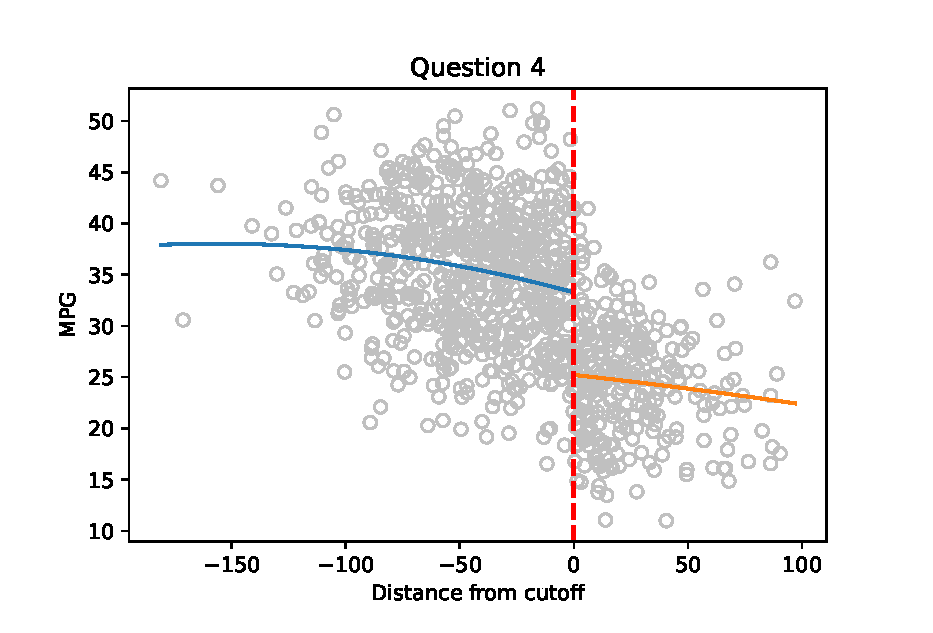
\includegraphics{hw8q4.eps}
\caption{Regression discontinuity estimates of the effect of the policy on fuel efficiency using a second-order polynomial.}
\label{fig:hw8q4}
\end{figure}

\begin{figure}[ht]
\centering
\includegraphics{hw8q5.eps}
\caption{Regression discontinuity estimates of the effect of the policy on fuel efficiency using a fifth-order polynomial.}
\label{fig:hw8q5}
\end{figure}

\end{document}